\chapter{Estado da Arte}
Ao decorrer desta pesquisa utilizamos como modelo de criptoativo o \textit{Bitcoin}, criado pelo pseudônimo Satoshi Nakamoto. Esta moeda é, atualmente, a mais estável diante do mercado de criptoativos e a mais antiga também, percorrendo desde 2008. É manifesto neste trabalho o contexto em que o \textit{Bitcoin} foi criado, seus objetivos diante da população e o detalhamento das tecnologias em que o ativo foi forjado.

Diante da tecnologia empregada no \textit{Bitcoin}, neste projeto é evidenciado os pilares principais em que se apoiam o desenvolvimento das criptomoedas, definido o trilema das criptos e como este trilema impacta na execução das suas determinadas funções.

Consta apresentado também o conceito de DeFi — Também entendido como finanças descentralizadas — e como este ecossistema tecnológico pode prover maior qualidade de vida e serviços para seus usuários.

Este projeto utiliza dos autores da Escola Austríaca de Economia — Ludwig von Mises, Böm Bawerk, Carl Menger, Friedrich Hayek e Murray Rothbard — para induzir a definição de dinheiro e moeda, pois, com foco na definição do conceito de dinheiro é possível argumentar o quão bem uma criptomoeda cumpre este papel em comparação com a moeda de curso legal do estado. 

\section{O Bitcoin} \label{sec:bitcoin}
O Bitcoin nasceu como um modelo de dinheiro digital que opera em uma rede descentralizada, sem a necessidade de uma autoridade central para emitir ou controlar a moeda. Foi proposto pela primeira vez em 2008 pelo programador não identificado conhecido como Satoshi Nakamoto, na documentação "Bitcoin: A Peer-to-Peer Electronic Cash System" \cite{Nakamoto2009} ,e lançado como software de código aberto em 2009. O Bitcoin permite transações peer-to-peer — de pessoa para pessoa e/ou ponto a ponto —, nas quais os usuários podem enviar e receber pagamentos diretamente, sem a necessidade de intermediários.

Este criptoativo é reconhecido por ser o primeiro e mais estável projeto de moeda digital e é definitivamente visto como referência de segurança, escalabilidade e descentralização no ambiente cripto.

Posteriormente há uma melhor definição da tecnologia de registro em que o Bitcoin atua, a Blockchain.

\section*{A Blockchain} \label{subsec:blockchain}
A tecnologia fundamental que sustenta o Bitcoin é a Blockchain, um livro-razão digital público e distribuído que registra todas as transações de forma transparente e imutável. A Blockchain é composta por blocos encadeados de forma cronológica. De maneria recursiva, cada bloco contém um conjunto — por ordem temporal — de transações confirmadas de maneira encadeada e um cabeçalho que inclui um hash do bloco anterior, formando assim uma cadeia de blocos interligados.

Na Figura \ref*{fig:blockchain} é possível visualizar o formato em que a estrutura de Blockchain é formada.

\begin{figure} [h]
    \centering
        \caption{Estrutura de encadeamento de blocos numa blockchain.}
        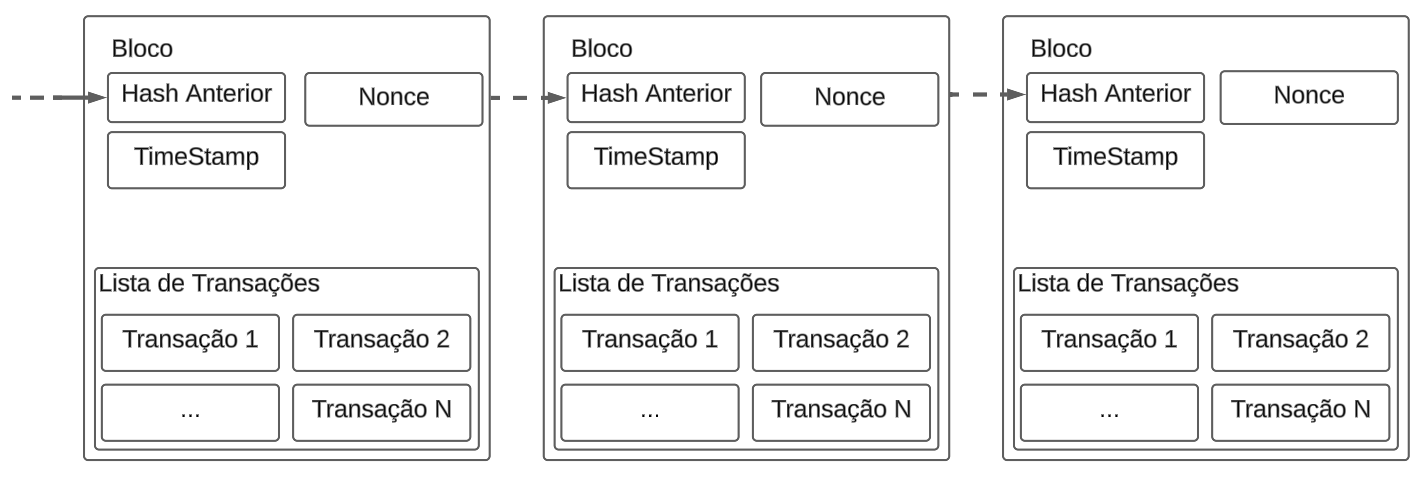
\includegraphics[width=.8\linewidth]{images/figura 2.png}
        \label{fig:blockchain}
        \text{Fonte: Tradução pelos autores, baseado na documentação de referência \cite{Nakamoto2009}}
\end{figure}

Na Figura \ref*{fig:transactions} é possível visualizar a estrutura de encadeamento das transações nos blocos.

\begin{figure} [h]
    \centering
        \caption{Encadeamento das transações nos blocos. Fonte: Os autores}
        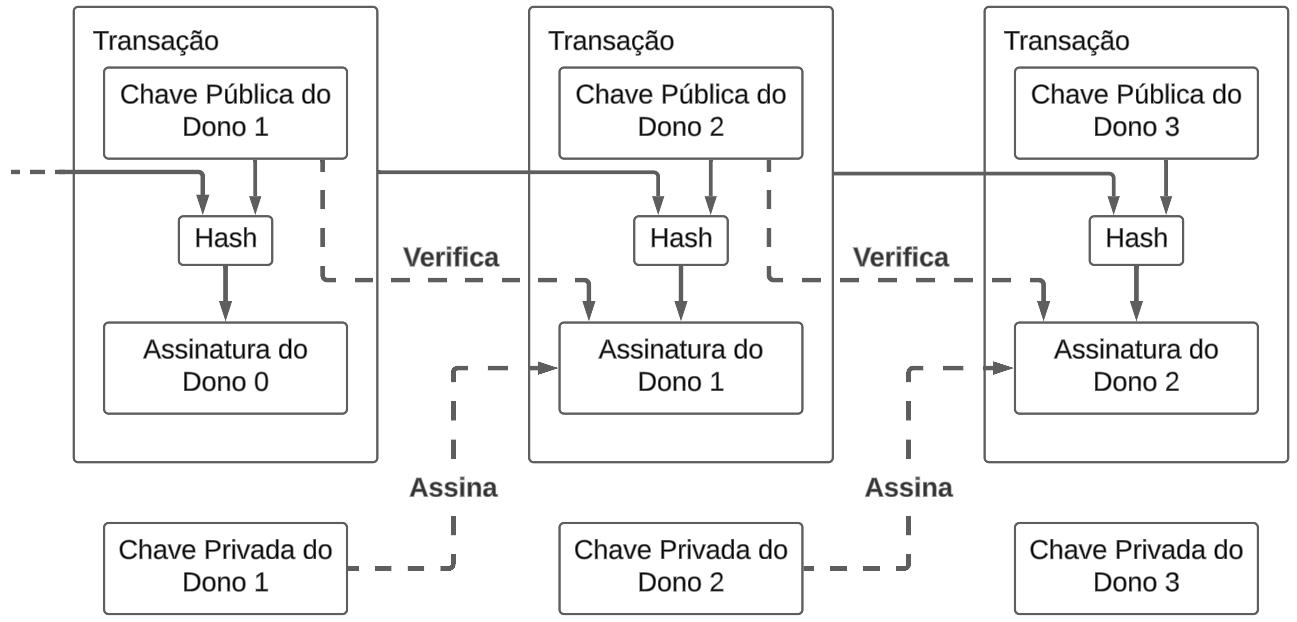
\includegraphics[width=.8\linewidth]{images/figura 1.png}
        \label{fig:transactions}
        \text{Fonte: Tradução pelos autores, baseado na documentação de referência \cite{Nakamoto2009}}

\end{figure} 

Em seguida é explicada a tecnologia de criptografia utilizada na atuação do Bitcoin.

\section*{Criptografia SHA-256 (Secure Hash Algorithm 256-bit)} \label{subsec:sha256}
O protocolo do Bitcoin emprega a criptografia SHA-256 (Secure Hash Algorithm 256-bit) como um componente fundamental para garantir a integridade e a segurança das transações na rede. Este algoritmo de hash criptográfico, desenvolvido pela Agência Nacional de Segurança (NSA) dos Estados Unidos e publicado pelo Instituto Nacional de Padrões e Tecnologia (NIST), é crucial para diversas operações dentro do ecossistema Bitcoin. 

O SHA-256 contribui para a segurança geral do protocolo Bitcoin por ser resistente a ataques de colisão e de pré-imagem, o que significa que é computacionalmente impraticável encontrar duas mensagens distintas que resultem no mesmo hash ou reverter um hash para obter a mensagem original. Essas propriedades são essenciais para manter a integridade das chaves e transações, garantindo que as entradas não possam ser manipuladas sem que isso seja facilmente detectado pela rede.

\section*{Algoritmo de Prova de Trabalho e Mineiração} \label{subsec:pow}
Para garantir a segurança e a integridade da Blockchain, o Bitcoin utiliza um algoritmo de consenso chamado Prova de Trabalho (tambem chamado de \textit{Proof of Work} ou PoW). Os mineradores coletam transações pendentes em um bloco e tentam gerar um \textit{hash} válido para esse bloco usando o SHA-256. 

A prova de trabalho se orienta dentro da blockchain diante do protocolo Merkle. O protocolo Merkle, também referido como árvore de Merkle ou \textit{hash} de Merkle, é uma estrutura de dados fundamental em criptografia, criada por Ralph Merkle. A árvore de Merkle ajuda a garantir que os dados não foram alterados, pois, qualquer modificação nos dados de entrada alteraria o \textit{hash} na folha correspondente e, por sua vez, todos os \textit{hashes} no caminho até a raiz.


O algoritmo é aplicado duas vezes (conhecido como double-SHA-256) ao cabeçalho do bloco, que inclui a versão do programa, o \textit{hash} do bloco anterior, o \textit{hash} Merkle das transações no bloco, o \textit{timestamp}, o nível de dificuldade e um \textit{nonce}. O termo \textit{nonce} refere-se a um número que é usado apenas uma vez (do inglês \textit{number used once}). O \textit{nonce} é um valor inteiro de 32 bits que os mineradores ajustam repetidamente para tentar produzir um \textit{hash} do bloco que atenda aos critérios de dificuldade estabelecidos pela rede Bitcoin.

O objetivo é encontrar um \textit{hash} que seja menor que o valor de dificuldade estabelecido pela rede, o que exige que os mineradores ajustem o \textit{nonce} repetidamente e recalculam o \textit{hash} do bloco até que um valor adequado seja encontrado. Este processo é fundamental para a implementação da prova de trabalho (Proof of Work - PoW), que ajuda a proteger a rede contra ataques.

\clearpage
\section{Escola Austríaca de Economia} \label{sec:austiaca}
O estudo da economia envolve a análise profunda de conceitos como economia, capital, dinheiro e crédito. Os economistas da Escola Austríaca, incluindo figuras proeminentes como Ludwig von Mises, Eugen Böhm von Bawerk, Carl Menger, Friedrich Hayek e Murray Rothbard, têm oferecido interpretações e teorias influentes que se diferenciam significativamente das abordagens mais tradicionais. 

\section*{Economia e a Ação Humana}
Ludwig von Mises, em sua obra "Ação Humana"\cite{von2023accao}, define economia como "a ciência que estuda a ação humana, uma aplicação da teoria do conhecimento humano". Segundo Mises, a economia é um ramo da praxeologia, ou seja, a teoria da ação humana. Ele argumenta que a economia, ao contrário de ser meramente uma análise de dados e tendências, é fundamentalmente sobre como os indivíduos escolhem agir com recursos escassos para atingir seus objetivos.

\section*{Capital segundo Böhm-Bawerk}
Eugen Böhm von Bawerk, um outro membro influente da Escola Austríaca, contribuiu significativamente para a teoria do capital. Em sua obra "Capital and Interest"\cite{von1922capital}, Böhm-Bawerk descreve o capital como "bens produzidos que servem como meios para a aquisição de bens futuros" (Böhm-Bawerk, 1884). Ele esclarece que o capital não é simplesmente uma acumulação de dinheiro ou ativos, mas sim ferramentas, máquinas e materiais que são usados para aumentar a produção futura.

\section*{Dinheiro e sua Origem para Menger}
Carl Menger, considerado o fundador da Escola Austríaca, foi um dos primeiros economistas a explicar a origem do dinheiro através de um processo de evolução social e não por decreto governamental ou convenção. Em sua obra "Princípios de Economia Política" \cite{menger2017liberalismo}, Menger argumentou que o dinheiro emergiu organicamente como o meio mais vendável de troca, facilitando assim as transações comerciais e reduzindo os custos de transação na economia (Menger, 1871).

\section*{Hayek e a Desestatização do Dinheiro}
Friedrich Hayek, ganhador do Prêmio Nobel, levou a teoria monetária austríaca para outra direção ao argumentar a favor da competição de moedas privadas em sua obra "Desnacionalização do Dinheiro" \cite{hayek2017desestatizaccao}. Hayek criticou os monopólios governamentais sobre a emissão de dinheiro, propondo que a concorrência entre diferentes categorias de dinheiro poderia prevenir a inflação e promover a estabilidade econômica.

\section*{A Teoria do Dinheiro de Mises}
Ludwig von Mises expandiu a teoria de Menger ao introduzir o conceito de "regressão" em sua análise do valor do dinheiro. Em "A Teoria do Dinheiro e do Crédito" \cite{von2013theory}, Mises apresenta a ideia de que o valor do dinheiro hoje é derivado da expectativa de seu poder de compra no futuro, que por sua vez é baseado em uma regressão contínua até o ponto em que o dinheiro era apenas um bem mais vendável entre outros (Mises, 1912). Mises também destacou o papel do dinheiro no cálculo econômico, essencial para a alocação racional de recursos em uma economia de mercado.

\section*{Rothbard e a Crítica à Moeda Fiduciária}
Murray Rothbard, seguindo a tradição de Mises, foi crítico em relação ao sistema de moeda fiduciária e ao papel dos bancos centrais. Em "O que o Governo fez com o Nosso Dinheiro?" \cite{rothbard2022governo}, Rothbard explica como o dinheiro historicamente ancorado em commodities, como o ouro, foi progressivamente substituído por dinheiro papel sem lastro, levando a ciclos econômicos mais instáveis e inflação.

\section{Bitcoin é dinheiro de verdade?} \label{sec:dinheiro}
Nesta secção, fazemos uma revisão do livro "Bitcoin, a moeda na era digital"\cite{Ulrich2014} escrito por Fernando Ulrich. O brasileiro é Mestre em Economia e referência por seu pioneirismo na divulgação de criptomoedas no Brasil. 

\section**{Definição Unificada de Dinheiro e Moeda}
Em seu livro, Ulrich chega a definição de moeda como "qualquer bem econômico empregado indefinidamente como meio de troca, independentemente de sua liquidez frente a outros bens monetários e de seus possíveis usos alternativos"\footnote{\cite{Ulrich2014} P.89}.

O autor lista atributos característicos a moeda, sendo eles sua escassez,
durabilidade, homogeneidade espacial e temporal, divisibilidade e maleabilidade, comparando o desempenho destes atributos diante do papel-moeda, o ouro e o Bitcoin, como mostra na Figura \ref*{fig:atributos}.

\begin{figure} [h]
    \centering
        \caption{Estrutura de encadeamento de blocos numa blockchain.}
        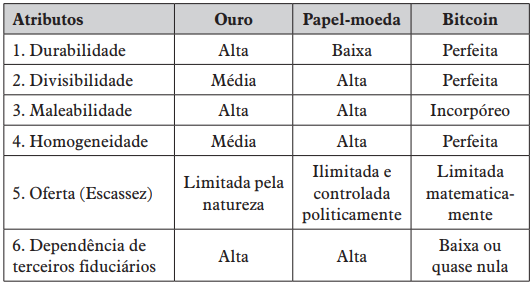
\includegraphics[width=.8\linewidth]{images/atributos.png}
        \label{fig:atributos}
        \text{Fonte: Bitcoin, a moeda na era digital; Ulrich,Fernando; 2014; p.67.}
\end{figure}

Ulrich menciona também as funções do dinheiro, listadas de servir como meio de troca, reserva de valor e unidade de conta. Em outras palavras, uma moeda deve servir, respectivamente, de maneira que as suas trocas sejam de forma facilitada; deve atuar de maneira em que possa ser entesourada e/ou guardada como reserva de riqueza; e por fim permita ser utilizável como meio de conta, utilizável ao cálculo econômico em função da moeda.

Segundo Fernando, o Bitcoin mostra-se capaz de performar as características e as funções da moeda tão bem, se não melhor, que o ouro e o papel-moeda. De acordo com ele "apesar da aparência unicamente digital, as atuais formas de dinheiro assemelham-se em muito ao Bitcoin. A maior parte da massa monetária no mundo moderno manifesta-se de forma intangível; nosso dinheiro já é um bem incorpóreo, uma característica que em nada nos impede de usá-lo diariamente"\footnote{Página 95}.

\section{Um Criptoativo Educativo} \label{sec:criptoeducativo}


% Descrição do estado da arte do tema. O estudante deve demonstrar conhecimento e embasamento. Entre 5 a 10 referências.
